\section{Derivation and approximation of Transparent Boundary Conditions for the linearized KdV equation}

\indent Two main objectives motivate the work developed in this section : firstly, we want to present the usual derivation of Transparent Boundary Conditions in the case of linearized problems; and secondly, after obtaining analytical expressions for the TBCs (which in general have a too much expensive application), we will propose, optimize and test approximations for them.

\subsection{Description of the TBCs}

\indent The derivation of the TBCs is based on \cite{besse2015} . We will consider the formulation for the continuous version of the homogeneous and linearized KdV equation :

\begin{equation}
\label{eq:kdv}
u_t + U_1u_x + U_2u_{xxx} = 0, \ \ U_1 \in \mathbb{R}, \ \ U_2 > 0
\end{equation}

\indent Denoting by $\laplinv$ the inverse Laplace transform, the TBCs are

\begin{equation}
\label{eq:TBC}
    \begin{cases}
        u(t,a) - U_2 \laplinv \left( \frac{\lambda_1(s)^2}{s} \right) * u_x(t,a) - U_2 \laplinv \left( \frac{\lambda_1(s)}{s} \right) * u_{xx}(t,a) = 0 \\
        u(t,b) - \laplinv \left( \frac{1}{\lambda_1(s)^2} \right) * u_{xx}(t,b) = 0 \\
        u_x(t,b) - \laplinv \left( \frac{1}{\lambda_1(s)} \right) * u_{xx}(t,b) = 0 
    \end{cases}
\end{equation}

\noindent where $[a,b]$ is the computational physical domain, $s \in \mathbb{C}$ is the Laplace frequency and $\lambda_1$ is one of the roots of the cubic characteristic equation obtained when solving \eqref{eq:kdv} in the Laplace space.

\indent We firstly notice that we can rewrite \eqref{eq:TBC} as

\begin{equation}
\label{eq:TBC2}
    \begin{cases}
        u(t,a) - U_2 \laplinv \left( \frac{\lambda_1(s)^2}{s} \hat{u}_x(t,s) \right)  - U_2 \laplinv \left( \frac{\lambda_1(s)}{s}  \hat{u}_{xx}(t,s) \right) = 0 \\
        u(t,b) - \laplinv \left( \frac{1}{\lambda_1(s)^2}   \hat{u}_{xx}(t,s) \right) = 0 \\
        u_x(t,b) - \laplinv \left( \frac{1}{\lambda_1(s)}   \hat{u}_{xx}(t,s) \right) = 0 
    \end{cases}
\end{equation}

\noindent where $\hat{u}$ is the Laplace transform of $u$.

\indent In the case of pure dispersion ($U_1 = 0$ and $U_2 = 1$), $\lambda$ is written as

$$ \label{eq:lambda} \lambda(s) = -\sqrt[3]{s} $$

\indent So, from \eqref{eq:lambda} we can write

\begin{equation}
    \label{eq:lambda2}
    \frac{\lambda}{s} = \frac{\lambda}{-\lambda^3} = -\frac{1}{\lambda^2} \\ 
    \frac{\lambda^2}{s} = \frac{\lambda^2}{-\lambda^3} = -\frac{1}{\lambda} \\
\end{equation}

\indent In the sequence, we will always consider this case ($U_1 = 0$ and $U_2 = 1$).



\subsection{Approximation of the TBCs}

\subsubsection{Approximation using a constant polynomial}

\indent In a first moment, we will approximate $\frac{\lambda^2}{s}$ by a constant polynomial $P_0(s) = c$. Therefore, from (\ref{eq:lambda2}) we get

\begin{equation}
    \frac{\lambda^2}{s} = c \\
    \frac{\lambda}{s} = -c^2 \\
    \frac{1}{\lambda_1(s)^2} = c^2 \\
    \frac{1}{\lambda_1(s)} = -c
\end{equation}

\noindent and replacing in (\ref{eq:TBC2}) and considering the linearity of the Laplace transform : 

\begin{equation}
\label{eq:TBC3}
    \begin{cases}
        u(t,a) - cU_2 u_x(t,a)  + c^2 U_2    u_{xx}(t,s) = 0 \\
        u(t,b) - c^2    \hat{u}_{xx}(t,s) = 0 \\
        u_x(t,b) + c u_{xx}(t,s)= 0 
    \end{cases}
\end{equation}

\indent Using finite difference approximations and considering different constants $c_L and c_R$ for the left and the right boundaries, (\ref{eq:TBC3}) is discretized as

\begin{equation}
\label{eq:TBC4}
    \begin{cases}
        u_0 - c_LU_2 \frac{u_1 - u_0}{\Delta x}  + c_L^2 U_2 \frac{u_0 -2u_1 + u_2}{\Delta x^2} = 0 \\
        u_N - c_R^2    \frac{u_N -2u_{N-1} + u_{N-2}}{\Delta x^2} = 0 \\
        \frac{u_N - u_{N-1}}{\Delta x}  + c_R^2    \frac{u_N -2u_{N-1} + u_{N-2}}{\Delta x^2} = 0 
    \end{cases}
\end{equation}



\subsubsection{Approximation using a linear polynomial}


\indent Similarly to the case presented above, we will approximate $\frac{\lambda^2}{s}$ by a linear polynomial $P_1(s) = ds + c$. Therefore,

\begin{equation}
    \frac{\lambda^2}{s} = ds + c \\
    \frac{\lambda}{s} = -(ds + c )^2 \\
    \frac{1}{\lambda_1(s)^2} = (ds + c )^2 \\
    \frac{1}{\lambda_1(s)} = -(ds + c )  
\end{equation}

\indent Thus, the inverse Laplace transforms in (\ref{eq:TBC2}) reads :

\begin{equation}
	\begin{split}
    \mathcal{L}^{-1} \left( \frac{\lambda^2}{s} \hat{u}_x(t,s) \right) = & \mathcal{L}^{-1} \left[ (ds+c) \hat{u}_x(t,s) \right] = \\
    			 & d\mathcal{L}^{-1} \left[ \hat{u}_{xt}(t,s) \right] + c \mathcal{L}^{-1} \left[ \hat{u}_{x}(t,s) \right] =   du_{xt}(x,t) + cu_x(x,t) \\
    \mathcal{L}^{-1} \left( \frac{\lambda}{s} \hat{u}_{xx}(t,s) \right) = & \mathcal{L}^{-1} \left[ -(ds+c)^2 \hat{u}_{xx}(t,s) \right] =  -d^2u_{xxtt}(x,t) -2dcu_{xxt}(x,t) - c^2u_{xx}(x,t) \\
    \mathcal{L}^{-1} \left( \frac{1}{\lambda^2} \hat{u}_{xx}(t,s) \right) = & \mathcal{L}^{-1} \left[ (ds+c)^2 \hat{u}_{xx}(t,s) \right] =d^2u_{xxtt}(x,t) + 2dcu_{xxt}(x,t) + c^2u_{xx}(x,t) \\
    \mathcal{L}^{-1} \left( \frac{1}{\lambda} \hat{u}_{xx}(t,s) \right) = & \mathcal{L}^{-1} \left[ -(ds+c) \hat{u}_{xx}(t,s) \right] = -du_{xxt}(x,t) - cu_{xx}(x,t)
    \end{split}
\end{equation}

\indent Using finite differences and different coefficients $c_L,c_R$ and $d_L,d_R$ for the left and the right boundaries, these expressions can be approximated by

\begin{equation}
    \label{eq:FDorder2A}
    \begin{split}
    \mathcal{L}^{-1} \left( \frac{\lambda^2}{s} \hat{u}_x(t,s) \right) = & d_L \frac{ (u_x)_0^{n+1} - (u_x)_0^n}{\Delta t} + c_L (u_x)_0^{n+1} = \\
    			& \left( \frac{d_L}{\Delta t} + c_L \right) \left( \frac{u_1^{n+1} - u_0^{n+1}}{\Delta x}\right) - \frac{d_L}{\Delta t} \left( \frac{u_1^{n} - u_0^{n}}{\Delta x}\right)
    \end{split}
 \end{equation}
 
 \begin{equation}
     \label{eq:FDorder2B}
    \begin{split}
    \mathcal{L}^{-1} \left( \frac{\lambda}{s} \hat{u}_{xx}(t,s) \right) = & -d_L^2 \left( \frac{(u_{xx})_0^{n+1} - 2(u_{xx})_0^{n} + (u_{xx})_0^{n-1}}{\Delta t^2} \right) + \\
    			&  - 2d_Lc_L \left( \frac{(u_{xx})_0^{n+1} - (u_{xx})_0^{n}}{\Delta t} \right) - c_L^2 (u_{xx})_0^{n+1} = \\
    			& -\left( \frac{d_L^2}{\Delta t^2} + \frac{2d_Lc_L}{\Delta t} + c_L^2  \right) \left(  \frac{u_0^{n+1} - 2u_1^{n+1} + u_2^{n+1}}{\Delta x^2} \right) + \\
    			& \left( 2\frac{d_L^2}{\Delta t^2} + \frac{2d_Lc_L}{\Delta t}\right) \left(  \frac{u_0^{n} - 2u_1^n + u_2^{n}}{\Delta x^2} \right) - \frac{d_L^2}{\Delta t^2} \left(  \frac{u_0^{n-1} - 2u_1^{n-1} + u_2^{n-1}}{\Delta x^2} \right)
    \end{split}
 \end{equation}
     			
\begin{equation}
     \label{eq:FDorder2C}
         \begin{split}
    \mathcal{L}^{-1} \left( \frac{1}{\lambda^2} \hat{u}_{xx}(t,s) \right) = & \left( \frac{d_R^2}{\Delta t^2} + \frac{2d_Rc_R}{\Delta t} + c_R^2  \right) \left(  \frac{u_{N}^{n+1} - 2u_{N-1}^{n+1} + u_{N-2}^{n+1}}{\Delta x^2} \right) + \\
    			& - \left( 2\frac{d_R^2}{\Delta t^2} + \frac{2d_Rc_R}{\Delta t}\right) \left(  \frac{u_N^{n} - 2u_{N-1}^n + u_{N-2}^{n}}{\Delta x^2} \right) + \\
    			& \frac{d_R^2}{\Delta t^2} \left(  \frac{u_N^{n-1} - 2u_{N-1}^{n-1} + u_{N-2}^{n-1}}{\Delta x^2} \right)
    \end{split}
 \end{equation}
     			
\begin{equation}
     \label{eq:FDorder2D}
         \begin{split}
    \mathcal{L}^{-1} \left( \frac{1}{\lambda} \hat{u}_{xx}(t,s) \right) = & -d_R \frac{ (u_{xx})_0^{n+1} - (u_{xx})_0^n}{\Delta t} - c_R (u_{xx})_0^{n+1} =\\
    			& -\left( \frac{d_R}{\Delta t} + c_R \right) \left( \frac{u_N^{n+1} -2 u_{N-1}^{n+1} + u_{N-2}^{n+1}}{\Delta x^2}\right) + \frac{d_R}{\Delta t}\left( \frac{u_{N}^{n} - 2u_{N-1}^{n} + u_{N-2}^n}{\Delta x^2}\right)
    \end{split}
\end{equation}

\indent Then we use \eqref{eq:FDorder2A} - \eqref{eq:FDorder2D} in \eqref{eq:TBC2} to obtain the discrete TBCs :

\begin{equation}
	\begin{split}
    u_0^{n+1} - U_2\left( \frac{d_L}{\Delta t} + c_L \right) \left( \frac{u_1^{n+1} - u_0^{n+1}}{\Delta x}\right) + \\
     U_2\left( \frac{d_L^2}{\Delta t^2} + \frac{2d_Lc_L}{\Delta t} + c_L^2  \right) \left(  \frac{u_0^{n+1} - 2u_1^{n+1} + u_2^{n+1}}{\Delta x^2} \right) = \\
     -U_2\frac{d_L}{\Delta t}\left( \frac{u_1^{n} - u_0^{n}}{\Delta x}\right) + U_2 \left( 2\frac{d_L^2}{\Delta t^2} + \frac{2d_Lc_L}{\Delta t}\right) \left(  \frac{u_0^{n} - 2u_1^n + u_2^{n}}{\Delta x^2} \right) + \\
     - U_2 \frac{d_L^2}{\Delta t^2} \left(  \frac{u_0^{n-1} - 2u_1^{n-1} + u_2^{n-1}}{\Delta x^2} \right)
   \end{split}
\end{equation} 

\begin{equation}
	\begin{split}
    u_N^{n+1} - \left( \frac{d_R^2}{\Delta t^2} + \frac{2d_Rc_R}{\Delta t} + c_R^2  \right) \left(  \frac{u_{N}^{n+1} - 2u_{N-1}^{n+1} + u_{N-2}^{n+1}}{\Delta x^2} \right) =\\
     -\left( 2\frac{d_R^2}{\Delta t^2} + \frac{2d_Rc_R}{\Delta t}\right) \left(  \frac{u_N^{n} - 2u_{N-1}^n + u_{N-2}^{n}}{\Delta x^2} \right) + \frac{d_R^2}{\Delta t^2} \left(  \frac{u_N^{n-1} - 2u_{N-1}^{n-1} + u_{N-2}^{n-1}}{\Delta x^2} \right)
    \end{split}
\end{equation} 
   
\begin{equation}
	\begin{split}	
    \frac{u_N^{n+1} - u_{N-1}^{n+1}}{\Delta x} + \left( \frac{d_R}{\Delta t} + c_R \right) \left( \frac{u_N^{n+1} -2 u_{N-1}^{n+1} + u_{N-2}^{n+1}}{\Delta x^2}\right) = \\
      \frac{d_R}{\Delta t}\left( \frac{u_{N}^{n} - 2u_{N-1}^{n} + u_{N-2}^n}{\Delta x^2}\right)
    \end{split}
\end{equation}


\subsection{Numerical tests}

\indent In order to validate compare our approximation with the results obtained by Besse, we will solve the same numerical test presented in his paper : 

\begin{equation}
\label{eq:Num1}
 u_t + u_{xxx} = 0, \ \ x \in \mathbb{R}
\end{equation}

\begin{equation}
\label{eq:Num2}
 u(0,x) = e^{-x^2}, \ \ x \in \mathbb{R} 
\end{equation}

\begin{equation}
\label{eq:Num3}
 u \rightarrow 0, \ \ |x| \rightarrow \infty
\end{equation}

\indent The fundamental solution of (\ref{eq:Num1}) is

\begin{equation}
    E(t,x) = \frac{1}{\sqrt[3]{3t}}Ai\left(\frac{x}{\sqrt[3]{3t}} \right)
\end{equation}

\noindent where $Ai$ is the Airy function, and the exact solution for the problem (\ref{eq:Num1}) - (\ref{eq:Num3}) is

\begin{equation}
    u_{exact}(t,x) = E(t,x) * e^{-x^2}
\end{equation}

\indent The problem will be solved in the spatial domain $[-6,-6]$

\indent For a quantitative evaluation of the results, we computed the same errors defined in the paper of Besse et al. For each time step, we compute the relative error

$$e^n = \frac{\left\Vert u_{exact}^n - u_{computed}^n\right\Vert_2}{\left\Vert u_{exact}^n\right\Vert_2}$$

\noindent and, in the whole time interval :

$$ e_{Tm} = \max\limits_{0 < n < T_{max}} (e^n) $$

$$ e_{L2} = \sqrt{ \Delta t \sum_{n=1}^{T_{max}} (e^n)^2 } $$

\indent We also generate plottings and animations for the best and the worst solutions. In order to make a better comparison, in the definition of "worst solution" we ignored the ones for which the numerical computations diverged (following the arbitrary criteria $e_{L2} > 10$.

\indent Several tests will be made with different combinations of the coefficients in the polynomial approximation of $\frac{\lambda^2}{s}$. For the constant polynomial $P_0(s) = c$, we will optimize the parameters $(c_L,c_R)$. For the linear polynomial $P_1(s) = cs+d$, we will optimize the four parameters $(c_L,d_L,c_R,d_R)$, but in a first moment we will consider $c_L = c_R$ and $d_L = d_R$ and study the behavior of the approximation in only one of the boundaries.


\subsection{Introduction tests}

\indent In a first moment, we will execute the tests with the proposed TBCs for a small range of parameters $(c_L,c_R)$ (for the constant polynomial approximation) and $(c_L,c_R,d_L,d_R)$ (for the linear polynomial approximation).  We tested all the possible combinations between the values in $[-10,-1,-0.1,0,0.1,1,10]$. In the case of the linear polynomial approximation, in order to avoid large computations, we considered only the cases where $c_L = c_R$ and $d_L = d_R$.

\indent The objective of these initial tests is to see the general behavior of the proposed approximations and guide our next steps in this study. The tables \ref{tab:firstTestsP0} and \ref{tab:firstTestsP1} show the best results (concerning the error $e_{L2}$) for each one of the approximations; and the figures \ref{fig:firstTestsP0} and \ref{fig:firstTestsP1} show some snapshots comparing the best, the worst and the analytical solution. The choice of the worst solution does not consider the ones that "exploded".

	 \sisetup{round-mode=places}
\begin{center}
\begin{tabular}{c|c|S[round-precision=4,table-number-alignment =  left]}
	\multicolumn{1}{c|}{$c_L$}  & \multicolumn{1}{c|}{$c_R$} & \multicolumn{1}{r}{$e_{L2}$} \\
	\hline
	1.0 & 1.0 & 0.0946839239675 \\
	1.0 & 10.0 & 0.097288371204 \\
	1.0 & 0.1 & 0.0983932287563 \\
	1.0 & 0.0 & 0.0992063806502 \\
	1.0 & -10.0 & 0.099359192771 \\
	1.0 & -0.1 & 0.100021589665 \\
	1.0 &  -1. & 0.10159265619 \\
	10.0 & 1.0 & 0.347003021321 \\
	10.0 & 0.1 & 0.347379492262 \\
	10.0 & 0.0 & 0.347487945035
\end{tabular}
\captionof{table}{Best results (smallest $e_{L2}$) for the constant polynomial approximation \label{tab:firstTestsP0}}
\end{center}


	 \sisetup{round-mode=places}
\begin{center}
\begin{tabular}{c|c|S[round-precision=4,table-number-alignment =  left]}
	\multicolumn{1}{c|}{$d_L = d_R$}  & \multicolumn{1}{c|}{$c_L = c_R$} & \multicolumn{1}{r}{$e_{L2}$} \\
	\hline
	0. & 1.0 & 0.0946839239675 \\
	0.1 & 1.0 & 0.12341195 \\
	1.0 & 1.0 & 0.20031603 \\
	10.0 & 0.1 & 0.22037249 \\
	-10.0 & 0.1 & 0.23984486 \\
	10.0 & 1.0 & 0.27161158 \\
	-10.0 &  0.0 & 0.24800816\\
	-10.0 & 1.0 & 0.30039637 \\
	10.0 & 0.0 & 0.27213611 \\
	0.0 & 0.1 & 0.36740764
\end{tabular}
\captionof{table}{Best results (smallest $e_{L2}$) for the linear polynomial approximation \label{tab:firstTestsP1}}
\end{center}

\noindent\begin{minipage}{\textwidth} 
	\begin{minipage}{.5\textwidth} 
		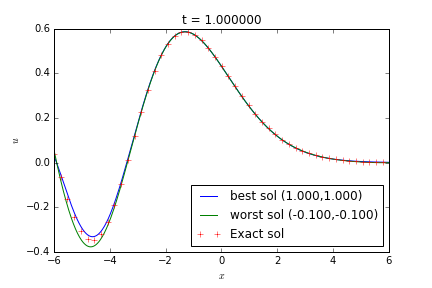
\includegraphics[scale=.48]{figures/TBCbesse/firstTestsP0Snap2.png}	
	\end{minipage}
	\begin{minipage}{.5\linewidth}
		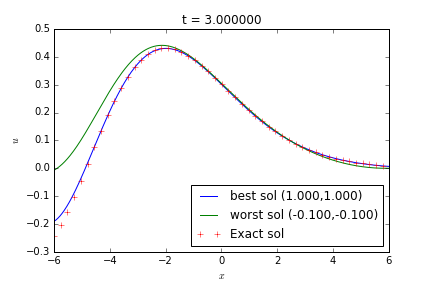
\includegraphics[scale=.48]{figures/TBCbesse/firstTestsP0Snap4.png}	
	\end{minipage}
	\captionof{figure}{Snapshots with the best and the worst solution in the case of the constant polynomial approximation \label{fig:firstTestsP0}}
\end{minipage}

\noindent\begin{minipage}{\textwidth} 
	\begin{minipage}{.5\textwidth} 
		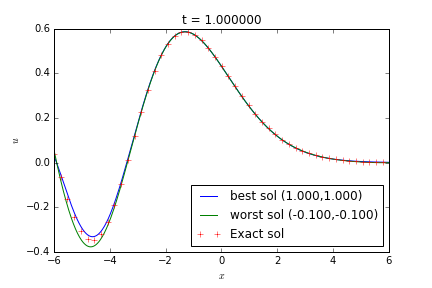
\includegraphics[scale=.48]{figures/TBCbesse/firstTestsP0Snap2.png}	
	\end{minipage}
	\begin{minipage}{.5\linewidth}
		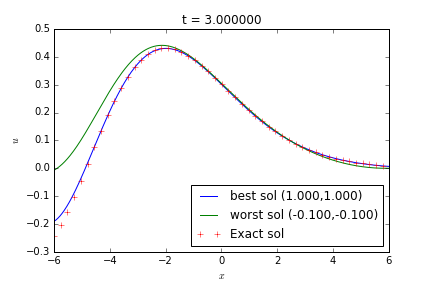
\includegraphics[scale=.48]{figures/TBCbesse/firstTestsP0Snap4.png}	
	\end{minipage}
	\captionof{figure}{Snapshots with the best and the worst solution in the case of the linear polynomial approximation \label{fig:firstTestsP1}}
\end{minipage}

\indent The results of the tables \ref{tab:firstTestsP0} and \ref{tab:firstTestsP1} and the figures \ref{fig:firstTestsP0} and \ref{fig:firstTestsP1} shows that using a higher-order polynomial approximation in the TBCs (which implies the existence of time derivative terms) does not improve the error of the numerical solution. In fact, the best solution was the one with $d_L = d_R = 0$, which leads to constant polynomial case. Additionally, The tests with $P_0$ shows that the solution is much more sensitive to the left than the right boundary, which is a consequence of the fact that the solution is practically constant and equal to zero in $L=6$, but shows great variations in $L=-6$.

\indent Therefore, in the following we will work only with the constant polynomial approximation, due to the better results that it provides and its simpler implementation.